\chapter{Time Series Discretization} \label{chap:ts_discretization}
One property of time series is that they often consist of a number of points that is too large to define data mining algorithms that work directly on the original time series, since their processing time would be intractable \cite{Survey_Esling}. As an example, consider that a day has 86,400 seconds. A sensor measurement every second would thus result in 86,400 time series points per day. This would add up to over 31 million time series points when measuring every day in a year. \newline
Therefore, algorithms are needed that transform time series into a representation with a reduced number of points while preserving their essential characteristics like extrema, anomalies and repeated patterns. Taking such a representation as the input for data mining algorithms would not only reduce the processing time, since it should meet all of the following requirements \cite{Survey_Esling}:
\vspace{-3pt}
\begin{enumerate}[itemsep=-10pt]
\item reduction of the number of time series points
\item extraction of the essential characteristics of the time series
\item computation of the representation with a lower processing time compared to the data mining algorithms
\item reconstruction of the original time series from the representation with high quality based on reconstruction error measures
\item implicit noise removal or insensitivity to noise
\end{enumerate}
\vspace{-3pt}
A representation that tries to meet these requirements is obtained by discretizing the original time series \cite{Survey_Temporal_Discretization}. The basic idea of such a discretization involves dividing the amplitude of the original time series into intervals based on breakpoints that are set at computed values along the amplitude. The discretized representation is then obtained by assigning each time series point to its respective interval and representing all points within an interval with the discrete value that is assigned to the interval (see Figure \ref{fig:time_series_discretization}).
\begin{figure}[htb]
\centering
\includegraphics[width=0.8\textwidth]{discretization/discretization.pdf}
\caption[Time Series Discretization - Basic Idea]{As an example, the amplitude of the plotted original time series is divided into four discretization intervals based on three breakpoints. The plotted discretization intervals are assigned the Latin letters \texttt{a}, \texttt{b}, \texttt{c}, and \texttt{d} as discrete values. For instance, all points of the original time series that are located in the \texttt{a}-discretization interval are assigned \texttt{a} to obtain the discretized representation of the original time series. The resulting discretized representation is then obtained by concatenating these discrete values in order of time the corrsponding points occur in the original time series \cite{Survey_Temporal_Discretization}. For the first five points this is \texttt{b}\texttt{c}\texttt{c}\texttt{c}\texttt{b}.}
\label{fig:time_series_discretization}
\end{figure}
\section{Piecewise Aggregate Approximation}
The algorithms for time series discretization explained in this chapter all depend on the \ac{PAA} as a preprocessing step. The \ac{PAA} first standardizes the original time series before it transforms it to an intermediate representation \cite{PAA_Keogh}. This intermediate representation is then used by the time series discretization algorithms to obtain the discretized representation of the original time series. \newline
\subsection*{Main Procedure}
Let $X = x_1, ..., x_N$ be a standardized time series of length $N \geq 1$. Further, consider X as a point in an $N$-dimensional space. Then, the main idea of the \ac{PAA} is to project X onto a lower-dimensional space of dimensionality $1 \leq n \leq N$ \cite{PAA_Keogh}. \newline
First, a non-overlapping sliding window of length $1 \leq w \leq N$ is used to partition $X$ into subsequences of equal length \cite{PAA_Keogh}. Assuming that $N$ is divisible by $w$, this results in $n = N \cdot w^{-1}$ subsequences of length $w$. The final step is to compute the mean of the $w$ points of each subsequence to get an approximation of the subsequence (see Figure \ref{fig:PAA}) \cite{PAA_Yi_Faloutsos}. \newline
Let $\overline{x}_i$ $(1 \leq i \leq n)$ be the mean of the $w$ points of the $i$-th extracted subsequence from $X$. Then, $\overline{X} = \overline{x}_1, ..., \overline{x}_n$ is the resulting time series in the lower-dimensional space of dimensionality $n$, where $\overline{x}_i$ is computed by \cite{PAA_Keogh}:
\begin{equation}
\overline{x}_i = \frac{n}{N} \sum_{j=\frac{N}{n}(i-1)+1}^{\frac{N}{n}i}\mkern-24mu x_j
\end{equation}
\begin{figure}[htb]
\centering
\includegraphics[width=0.8\textwidth]{discretization/paa/paa_sliding_window_short.pdf}
\caption[Piecewise Aggregate Approximation - Sliding Window]{The original time series is partitioned by a non-overlapping sliding window into subsequences of equal length. For each subsequence the mean of its points is computed. These means (green squares) are the points of the time series that is the result of the \ac{PAA} \cite{PAA_Keogh}.} 
\label{fig:PAA}
\end{figure}
\subsection*{Strategies for Time Series of Indivisable Length}
The assumption that $N$ is divisible by $w$ is not a requirement of the \ac{PAA}, but it simplifies notation and understanding \cite{PAA_Keogh}. \newline
One strategy when $N$ is not divisible by $w$ is to append additional points with a value of zero to $X$ until $N$ is divisible by $w$ \cite{PAA_Yi_Faloutsos}. This is a straightforward strategy. But, on the other hand, the mean computed for the last extracted subsequence will be distorted. The extent of this distortion will be greater the closer the number of additionally appended points is to $w$. \newline
Another strategy is to truncate the points of $X$ until $N$ is divisible by $w$. This is also a straightforward strategy, but the time series is modified and information, in the form of time series points, is lost. \newline
The strategy that is used for the evaluation in this thesis (see Chapter \ref{evaluation_chapter}) tries to find a compromise between the strategies mentioned above. First, the window length $w$ is applied on the time series. Then, depending on the number of points contained in the last extracted subsequence, it is decided to truncate these points or to compute the mean of these points. When this number of points is greater than $\frac{w}{2}$, the mean of these points is computed, otherwise these points along with the last extracted subsequence are truncated. Due to this threshold of $\frac{w}{2}$, this strategy is straightforward, does not distort the mean computed for the last extracted subsequence, and limits the loss of information.
\subsection*{Role of the Window Length as Input Parameter} \label{parameter_window_length}
Since the \ac{PAA} is a downsampling approach, $\overline{X}$ is an approximation of $X$ which incurs a loss of information \cite{PAA_Yi_Faloutsos}. On the other hand, this approximation also incurs a gain in free memory. From $n \leq N$ it follows that storing $\overline{X}$ needs at most as much memory as storing $X$. These two observations imply a trade-off between the loss of information and the gain in free memory incurred when applying the \ac{PAA} on $X$ \cite{SAX_Lin}. \newline
The decisive parameter that affects this trade-off is the window length $w$ \cite{SAX_Lin}. Qualitatively, as $w$ increases more information is lost, but less memory for storing $\overline{X}$ is required, because less means $\overline{x}_i$ are computed to approximate $X$. On the other hand, as $w$ decreases less information is lost, but more memory for storing $\overline{X}$ is required, because more means $\overline{x}_i$ are computed to approximate $X$. When assigning each point of an extracted subsequence the corresponding mean of the subsequence, this trade-off can be visualized (see Figure \ref{fig:PAA_inverse}) \cite{SAX_Lin}. \newline
Note that $\overline{X}$ is the mean of $X$ for the extreme case of $w = N$ and $\overline{X} = X$ for the extreme case of $w = 1$, meaning that each point of $X$ is its own mean \cite{PAA_Keogh}.
\begin{figure}[htb]
\centering
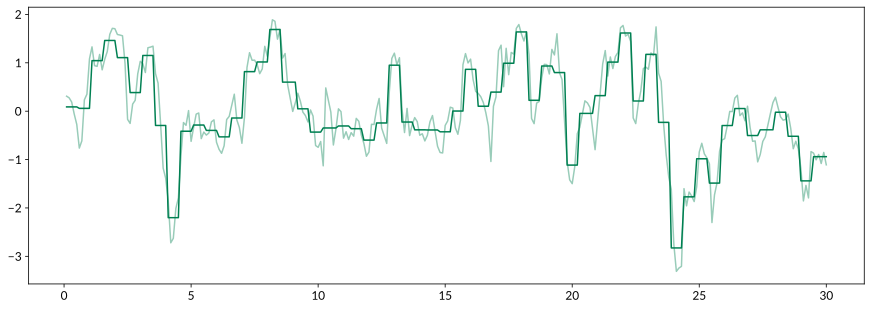
\includegraphics[width=0.8\textwidth]{discretization/paa/paa_inverse_transformation.pdf}
\caption[Piecewise Aggregate Approximation - Effect of Window Size]{The original time series in these two plots consists of 300 points. In the plot above a window length of $w = 5$ (i.e. five points) is used to extract the subsequences, while in the plot below a window length of $w = 10$ (i.e. ten points) is used. The approximation in the plot above captures more fine-grained characteristics of the original time series like local extrema, while the approximation in the plot below is more coarse-grained. However, the approximation in the plot above is created with 60 points (i.e means) compared to 30 points (i.e. means) that are used for the approximation in the plot below.} 
\label{fig:PAA_inverse}
\end{figure}
\subsection*{Time Complexity}
For the \ac{PAA}, $\frac{N}{w}$ subsequences need to be extracted from $X$ while each subsequence contains $w$ points. Further, the computation of the mean is linear in the number of points. Hence, the \ac{PAA} has a time complexity of $\mathcal{O}(\frac{N}{w}\cdot w) = \mathcal{O}(N)$ \cite{PAA_Keogh}.

\newpage
\section{Fixed-breakpoints Discretization}
The following three time series discretization algorithms all assume that the original time series that shall be discretized follow the standard normal distribution $\mathcal{N}(0,1)$ after applying standardization \cite{SAX_Lin}. Based on this assumption, the breakpoints that define the discretization intervals along the amplitude of the time series are computed by the quantiles of the standard normal distribution \cite{SAX_Lin}. Thus, given a fixed number of discretization intervals to be used, all time series are discretized based on the same breakpoints. Therefore, the breakpoints are not adaptive to the time series data at hand, which is the reason the following three discretization algorithms are classified into fixed-breakpoints discretization.
\newpage
\subsection{Symbolic Aggregate Approximation}
The \ac{SAX} discretization algorithm applies amplitude discretization to the \ac{PAA} representation to obtain the discretized \ac{SAX} representation of the original time series \cite{SAX_Lin}. Due to the fixed breakpoints discussed above, every \ac{PAA} representation is discretized based on the same discretization intervals.
\subsection*{Main Procedure}
Let $X = x_1, ..., x_N$ be a standardized time series of length $N \geq 1$. Assume that $X$ follows the standard normal distribution $X \sim \mathcal{N}(0,1)$. Further, define $P := \{\frac{j}{a} \mid j \in \{1, ..., a-1\}\}$ for a given natural number $a \geq 2$. Applying the quantile function of the standard normal distribution to the probabilities in $P$ results in the $a$-quantiles $\beta_j \ (1 \leq j \leq a-1)$ of the standard normal distribution. The ascending sorted list of these $a$-quantiles $B := (\beta_0, \beta_1, ..., \beta_{a-1}, \beta_a)$ with $\beta_0 = -\infty$ and $\beta_a = +\infty$ are called breakpoints and $a$ is called alphabet size \cite{SAX_Lin_first}. Define $A := \{\alpha_j \mid j \in \{1, ..., a\}\}$ as the corresponding alphabet with $a$ symbols (e.g. letters from the Latin alphabet). \newline
Discretizing $X$ now first requires its transformation into its \ac{PAA} representation $\overline{X} = \overline{x}_1, ..., \overline{x}_n$ with $1 \leq n \leq N$. Then, the discretized \ac{SAX} representation $\hat{X} = \hat{x}_1, ..., \hat{x}_n$ of $X$ is obtained by mapping the means $\overline{x}_i$ to alphabet symbols $\alpha_j$ \cite{SAX_Lin_first}:
\begin{equation}
\hat{x}_i = \alpha_j \iff \beta_{j-1} \leq \overline{x}_i < \beta_j \qquad (1 \leq i \leq n, \; 1 \leq j \leq a)
\label{eq:SAX_Discretization}
\end{equation}
Hence, all means $\overline{x}_i$ of the \ac{PAA} representation of $X$ that are smaller than the breakpoint $\beta_1$ are mapped to the alphabet symbol $\alpha_1$, all means that are greater than or equal to the breakpoint $\beta_1$ and smaller than the breakpoint $\beta_2$ are mapped to the alphabet symbol $\alpha_2$ and so on (see Figure \ref{fig:SAX_discretization}) \cite{SAX_Lin_first}. Therefore, the discretization intervals along the amplitude are defined by $[\beta_{j-1},\beta_j) \ (1 \leq j \leq a)$. \newline
Further, note that the breakpoints $\beta_j$ split the standard normal distribution into $a$ areas, each containing $\frac{1}{a}$ of the total area under the curve, given their definition as $a$-quantiles of the standard normal distribution \cite{SAX_Lin_first}.
\begin{figure}[htb]
\centering
\includegraphics[width=0.8\textwidth]{discretization/sax/discretization.pdf}
\caption[Symbolic Aggregate Approximation - Discretization]{The original time series is discretized based on its PAA representation with an alphabet size of $a = 4$. It is assumed that the original time series follows the standard normal distribution $\mathcal{N}(0,1)$. Based on this assumption the discretization intervals along its amplitude are determined \cite{SAX_Lin_first}. Using lowercase letters from the Latin alphabet for the alphabet symbols, the resulting discretized representation of the original time series is: \textcolor{red}{bcddcdbaaaabcbbbbaa}.}
\label{fig:SAX_discretization}
\end{figure}
\subsection*{Role of the Alphabet Size as Input Parameter} \label{parameter_alphabet_size}
From the definition of the breakpoints as $a$-quantiles of the standard normal distribution, it follows that the alphabet size $a$ is equal to the number of discretization intervals. Furthermore, if the alphabet size $a$ increases the distance $\beta_j - \beta_{j-1}$ between two adjacent breakpoints decreases, because each discretization interval $[\beta_{j-1}, \beta_j)$ covers $\frac{1}{a}$ of the area under the curve of the standard normal distribution \cite{SAX_Lin_first}. Therefore, the range of continuous values that each alphabet symbol covers becomes narrower when the alphabet size $a$ increases. \newline
Assuming that the means $\overline{x}_i \ (1 \leq i \leq n)$ of the \ac{PAA} representation $\overline{X}$ follow the standard normal distribution, each discretization interval contains $\frac{1}{a}$ of the total number of means $\overline{x}_i$. Thus, the number of means in each discretization interval decreases when the alphabet size $a$ increases. \newline
Hence, the alphabet size $a$ controls the granularity of the discretization of the means $\overline{x}_i$ \cite{SAX_Lin}. Meaning that the greater the alphabet size, the more likely it is that each different mean is assigned a different alphabet symbol when discretizing. In other words, it is more likely that each different mean is assigned its own unique alphabet symbol. \newline
This effect can be even more extreme when considering a small window length used in the \ac{PAA}. For example, consider a window length of $w = 1$. Then it is $\overline{X} = X$, meaning that each point in $X$ is its own mean. Further, suppose an alphabet size of $\lim_{a \to +\infty} a$. Assuming that $X$ does not contain any duplicate values, it follows that each point $x_i \ (1 \leq i \leq N)$ of $X$ is assigned its own unique alphabet symbol when discretizing. \newline
All in all, increasing the alphabet size results in a more granular discretization of the means of the \ac{PAA} representation and vice versa (see Figure \ref{fig:SAX_alphabet_size}). However, increasing the alphabet size also results in increased memory requirements for storing the \ac{SAX} representation $\hat{X}$, because the more alphabet symbols used the greater the memory requirement per symbol. Therefore, a trade-off dependent on the alphabet size exists between the granularity of the discretization and the memory requirements of the \ac{SAX} representation of the original time series \cite{SAX_Lin}.
\begin{figure}[htb]
\centering
\includegraphics[width=0.8\textwidth]{discretization/sax/sax_alphabet_density.pdf}
\caption[Symbolic Aggregate Approximation - Effect of Alphabet Size]{In the left plot, the breakpoints for an alphabet size of $a = 5$ are shown. In the right plot, the breakpoints for an alphabet size of $a = 8$ are shown. For instance, the range of continuous values the alphabet symbol \textcolor{red}{c} covers is narrower for $a = 5$ compared to $a = 8$. Thus, the discretization shown in the right plot is more granular by using more alphabet symbols.}
\label{fig:SAX_alphabet_size}
\end{figure}
\subsection*{Distance Measures}
One usage of distance measures in the context of time series is to measure the similarity between a given time series and each time series stored in a database in order to retrieve similar time series from it \cite{Survey_Esling}. There are two reasons why such a procedure is more time efficient with \ac{SAX} representations than  with the corresponding original time series. \newline
The first reason is that time series databases storing original time series are more likely to need to be stored on disk while those storing \ac{SAX} representations are more likely to be held in main memory due to less memory requirements \cite{SAX_Lin}. Therefore, accessing \ac{SAX} representations is more likely to be faster than accessing original representations. \newline
The second reason is that the time efficiency of distance computations between two time series is dependent on the number of points these time series have. Therefore, distance computations between \ac{SAX} representations are more likely to be faster than between the corresponding original time series due to less number of points respectively alphabet symbols \cite{SAX_Lin}. \newline
For these two reasons, the following time efficient procedure can be applied based on \ac{SAX} representations \cite{SAX_Lin, Faloutsos_Bounding_Lemma}. \newline
Suppose two time series databases $DB := \{X \mid X \ time \ series \ of \ length \ N \geq 1\}$ and $DB^{SAX} := \{\hat{X} \mid X \in DB\}$ where each time series $X$ is stored in its \ac{SAX} representation $\hat{X}$ of length $ 1 \leq n \leq N$.  Further, assume that $DB$ is stored on disk while $DB^{SAX}$ is held in main memory due to less memory needed for $DB^{SAX}$ than for $DB$. \newline
Now given a time series $X^*$ of length $N$, the set of time series 
\begin{center}
$DB^* := \{X \mid X \in DB, \ Eucl(X^*, X) \leq r\}$
\end{center}
shall be found, where $Eucl$ is the Euclidean distance between two original time series and $r \geq 0$ is a given real number distance. The Euclidean distance is assumed to be the true distance between two original time series and is one possible distance measure for this procedure \cite{Survey_Esling}. \newline
The first step for finding $DB^*$ is to discretize $X^*$ based on the \ac{SAX} in order to be able to compare its \ac{SAX} representation $\hat{X}^*$ with the \ac{SAX} representations in $DB^{SAX}$. \newline
The next step is to define a distance measure $MINDIST$ that measures the distance between any two \ac{SAX} representations and lower-bounds the Euclidean distance for the corresponding original time series (see Figure \ref{fig:Euclidean_Mindist}):
\begin{equation}
MINDIST(\hat{X}^*,\hat{X}) \leq Eucl(X^*,X)
\label{eq:lowerBounding}
\end{equation}
With $MINDIST$, the \ac{SAX} representations in $DB^{SAX}$ can be filtered by discarding those that definitely do not fullfill $Eucl(X^*,X) \leq r$. Then, the resulting filtered database is $DB^{SAX'} := \{\hat{X} \mid \ X \in DB, \ MINDIST(\hat{X}^*,\hat{X}) \leq r\}$. This filtering property of $MINDIST$ follows from Equation \ref{eq:lowerBounding}, because each $\hat{X} \in DB^{SAX}$ with $MINDIST(\hat{X}^*,\hat{X}) > r$ can be neglected, since it is:
\begin{center}
$MINDIST(\hat{X}^*,\hat{X}) > r \implies Eucl(X^*,X) > r$
\end{center}
Equation \ref{eq:lowerBounding} also guarantees no false dismissals during this filtering process. Hence, there is no $\hat{X} \in DB^{SAX}$ that is filtered out, but fullfills $Eucl(X^*,X) \leq r$. This property of $MINDIST$ is known as the Lower Bounding Lemma \cite{Faloutsos_Bounding_Lemma}. \newline
However, after this filtering process there can be still some $\hat{X} \in DB^{SAX'}$ where $Eucl(X^*,X) > r$ holds, because $MINDIST$ underestimates the Euclidean distance according to Equation \ref{eq:lowerBounding}. \newline
Hence, the last step to find $DB^*$ is to filter these false positives out of $DB^{SAX'}$. This is done by retrieving the original time series $X$  of all $\hat{X} \in DB^{SAX'}$ from $DB$ and computing $Eucl(X^*,X)$. $DB^*$ then results from keeping each $X \in DB$ that fulfills $Eucl(X^*,X) \leq r$. \newline
Note that only during this last step, the original time series $X$ are retrieved from $DB$ that is stored on disk. Further, not every $X \in DB$ is retrieved, but only those that are in the filtered $DB^{SAX'}$. Before this last step, the distances are computed on the \ac{SAX} representations $\hat{X}$ based on $MINDIST$. These \ac{SAX} representations are held in main memory and are represented by less number of alphabet symbols compared to the number of points of the original time series. \newline
The question that now remains is what distance measure $MINDIST$ that lower-bounds the Euclidean distance shall be used. One important characteristic of the \ac{SAX} is that it provides such a lower bounding distance measure. It is defined as \cite{SAX_Lin}:
\begin{equation}
MINDIST(\hat{X},\hat{Y}) := \sqrt{\frac{N}{n}}\sqrt{\sum_{i=1}^{n} (dist(\hat{x}_i, \hat{y}_i))^2}
\label{eq:mindist}
\end{equation}
where $\hat{X} = \hat{x}_1, ..., \hat{x}_n$ and $\hat{Y} = \hat{y}_1, ..., \hat{y}_n$ are the \ac{SAX} representations with $n$ alphabet symbols of the original time series $X$ and $Y$ of length $N$, respectively. The subfunction $dist$ is defined for $1 \leq i,j \leq a$ as:
\begin{equation}
dist(\alpha_i, \alpha_j) :=
\begin{cases}
0, & \text{if } |i - j| \leq 1 \\
\beta_{\max \{i,j\}-1} - \beta_{\min \{i,j\}}, & \text{otherwise}
\end{cases}
\label{eq:dist}
\end{equation}
where $\alpha_i, \alpha_j$ are alphabet symbols and $\beta_i, \beta_j$ are breakpoints.
\begin{figure}[htb]
\centering
\includegraphics[width=0.8\textwidth]{discretization/sax/euclidean_mindist.pdf}
\caption[Symbolic Aggregate Approximation - Euclidean vs. MINDIST]{In the plot above, the Euclidean distance is indicated by connecting each pair of points of the original time series $X^*$ and $X$ that belong to the same point in time \cite{SAX_Lin}. Below this plot, the $MINDIST$ of the corresponding \ac{SAX} representations $\hat{X}^*$ and $\hat{X}$ is indicated by connecting the pairwise symbols whose distance shall be measured \cite{SAX_Lin}. The $MINDIST$ shall lower-bound the Euclidean distance: $MINDIST(\hat{X}^*, \hat{X}) \leq Eucl(X^*, X)$.}
\label{fig:Euclidean_Mindist}
\end{figure}
\subsection*{Time Complexity}
The first step of the \ac{SAX} involves the computation of the breakpoints. A static lookup table that contains the $a$-quantiles of the standard normal distribution can be used to retrieve the ascending sorted breakpoints for a given alphabet size $a$ \cite{SAX_Lin}. Thus, the time complexity for computing the breakpoints for a given alphabet size is $\mathcal{O}(1)$. Note that the breakpoints $\beta_0 = -\infty$ and $\beta_a = +\infty$ are not actually needed. Therefore, $a$ alphabet symbols can be represented by $a-1$ breakpoints. \newline
The final step is to map each of the $n$ means of the \ac{PAA} representation to one alphabet symbol. Based on the retrieved ascending sorted breakpoints, a binary search can be applied for the mapping of each mean. Thus, the time complexity for this step is $\mathcal{O}(n \cdot log_{2}(a-1)) = \mathcal{O}(n)$ for a given alphabet size $a$. \newline
Therefore, the time complexity of the discretization process with the \ac{SAX} is $\mathcal{O}(n)$.
Taken the time complexity of $\mathcal{O}(N)$ of the \ac{PAA} into account, the total time complexity of the \ac{SAX} is $\mathcal{O}(n) + \mathcal{O}(N) = \mathcal{O}(N)$, because it is $N \geq n$ \cite{SFA}.
\subsection{Extended Symbolic Aggregate Approximation}
Similar to the \ac{SAX}, the \ac{eSAX} discretization algorithm applies amplitude discretization to the \ac{PAA} representation in order to obtain the discretized \ac{eSAX} representation of the original time series \cite{E_SAX}. Moreover, the \ac{eSAX} uses the same fixed breakpoints as the \ac{SAX} for computing the discretization intervals along the amplitude. \newline
However, the \ac{eSAX} does not use the same \ac{PAA} version as the \ac{SAX}, but modifies it in order to extract two additional characteristic values from each subsequence that is extracted by the sliding window \cite{E_SAX}. With these two additional characteristic values, the trend of the points of a subsequence shall be captured.
\subsection*{Main Procedure}
Let $X = x_1, ..., x_N$ be a standardized time series of length $N \geq 1$ that follows the standard normal distribution $X \sim \mathcal{N}(0,1)$. The first step of discretizing $X$ based on the \ac{eSAX} is to apply a modified version of the PAA on $X$ \cite{E_SAX}. In addition to computing the mean, the minimum as well as the maximum point of the points in each sliding window are retrieved. Hence, the resulting \ac{PAA} representation of this modified version can be represented by $X' = \{min_1, \overline{x}_1, max_1\}, ..., \{min_n, \overline{x}_n, max_n\}$, where $1 \leq n \leq N$ and $\{min_i, \overline{x}_i, max_i\}$ $(1 \leq i \leq n)$ is the minimum point, mean, and maximum point of the points of the $i$th extracted subsequence by the sliding window, respectively. \newline
In the next step of the \ac{eSAX}, these computed means along with the minima and maxima are then discretized analogous to the \ac{SAX} discretization based on Equation \ref{eq:SAX_Discretization} \cite{E_SAX}. The resulting time series after this step can then be represented by $X'' = \{\hat{min_1}, \hat{x}_1, \hat{max_1}\}, ..., \{\hat{min_n}, \hat{x}_n, \hat{max_n}\}$, where $\{\hat{min_i}, \hat{x}_i, \hat{max_i}\}$ are the alphabet symbols for the minimum point, mean, and maximum point, respectively. Thus, the \ac{eSAX} accounts for extreme points within a subsequence that are middled out in the \ac{SAX} discretization (see Figure \ref{fig:SAX_E_SAX}) \cite{E_SAX}. \newline
However, $X''$ is not the final discretized \ac{eSAX} representation, because the positions of $\hat{min_i}$ and $\hat{max_i}$ in the \ac{eSAX} representation shall correspond to the positions of the corresponding $min_i$ and $max_i$ within $X$ with respect to the point in time they occur \cite{E_SAX}. \newline
Therefore, the last step of the \ac{eSAX} involves sorting each $\{\hat{min_i}, \hat{x}_i, \hat{max_i}\}$ according to the positions in time of the corresponding $\{min_i, \overline{x}_i, max_i\}$ within $X$ \cite{E_SAX}. Thus, the final discretized \ac{eSAX} representation can be represented by $\hat{X} = sort(\{\hat{min_1}, \hat{x}_1, \hat{max_1}\}), ..., sort(\{\hat{min_n}, \hat{x}_n, \hat{max_n}\})$ (see Figure \ref{fig:E_SAX}), where the function $sort$ is described by \cite{E_SAX}:
\begin{algorithmic}
\STATE 1. Compute the positions $t(min_i)$, $t(\overline{x}_i)$, and $t(max_i)$ in time within $X$. The position of $\overline{x}_i$ is computed by 
\begin{center}
$t(\overline{x}_i) = \frac{t(s_i^1) \;+\; t(s_i^w)}{2}$,
\end{center}
where $t(s_i^1)$ and $t(s_i^w)$ is the starting and ending position in time of the $i$th extracted subsequence within $X$ based on a window length of $w \geq 1$.
\STATE 2. Sort $\hat{min_i}$, $\hat{max_i}$, and $\hat{x_i}$ in ascending order based on the corresponding computed positions in 1.
\STATE 3. Return the sorted values.
\end{algorithmic}
Since $min_i$ and $max_i$ can be arbitrarily located in the $i$th extracted subsequence of $X$, $sort(\{\hat{min_i}, \hat{x}_i, \hat{max_i}\})$ can have $3! = 6$ different return values, namely every permutation of $\{\hat{min_i}, \hat{x}_i, \hat{max_i}\}$ \cite{E_SAX}.
\subsection*{Time Complexity}
In the modified version of the  \ac{PAA} that is used for the \ac{eSAX}, the minimum and maximum for each extracted subsequence can be computed along with the mean in linear time. Therefore, the time complexity of the modified version of the \ac{PAA} remains $\mathcal{O}(N)$. \newline
Since for the \ac{eSAX} three values need to be discretized for each of the $n$ extracted subsequences, the time complexity for the discretization process is $\mathcal{O}(3n \cdot log_{2}(a-1))$ compared to $\mathcal{O}(n \cdot log_{2}(a-1))$ for the \ac{SAX}, where $a \geq 2$ is the fixed alphabet size used for discretizing. \newline
As a last step, the minimum, maximum, and mean needs to be sorted for each of the $n$ extracted subsequences. This can be done in $\mathcal{O}(3 \cdot log_{2}(3) \cdot n)$. \newline
Therefore, the total time complexity of the \ac{eSAX} with the time complexity of the \ac{PAA} is $\mathcal{O}(N) + \mathcal{O}(3n \cdot log_{2}(a-1)) + \mathcal{O}(3 \cdot log_{2}(3) \cdot n) = \mathcal{O}(N) + \mathcal{O}(n) + \mathcal{O}(n) = \mathcal{O}(N)$, because it is $N \geq n$.
\begin{figure}[htb]
\centering
\includegraphics[width=0.8\textwidth]{discretization/e_sax/e_sax_vs_sax.pdf}
\caption[Extended Symbolic Aggregate Approximation - SAX vs. eSAX]{Based on the alphabet symbols $a$, $b$, $c$ and a window length of $w = 5$, the \ac{SAX} representation in the above plot is \textcolor[rgb]{0,0.39,0}{b} \textcolor[rgb]{0,0.39,0}{b} \textcolor[rgb]{0,0.39,0}{b} \textcolor[rgb]{0,0.39,0}{b} \textcolor[rgb]{0,0.39,0}{b} \textcolor[rgb]{0,0.39,0}{b} for the original time series. On the other hand, the \ac{eSAX} representation in the below plot does not middle out the extreme points within a subsequence and captures the actual pattern of the original time series \cite{E_SAX}: \textcolor[rgb]{0,0,0.39}{a}\textcolor[rgb]{0,0.39,0}{b}\textcolor{orange}{c} \textcolor{orange}{c}\textcolor[rgb]{0,0.39,0}{b}\textcolor[rgb]{0,0,0.39}{a} \textcolor[rgb]{0,0,0.39}{a}\textcolor[rgb]{0,0.39,0}{b}\textcolor{orange}{c} \textcolor{orange}{c}\textcolor[rgb]{0,0.39,0}{b}\textcolor[rgb]{0,0,0.39}{a} \textcolor[rgb]{0,0,0.39}{a}\textcolor[rgb]{0,0.39,0}{b}\textcolor{orange}{c} \textcolor{orange}{c}\textcolor[rgb]{0,0.39,0}{b}\textcolor[rgb]{0,0,0.39}{a}.}
\label{fig:SAX_E_SAX}
\end{figure}
\begin{figure}[htb]
\centering
\includegraphics[width=0.8\textwidth]{discretization/e_sax/e_sax.pdf}
\caption[Extended Symbolic Aggregate Approximation - Discretization]{For the \ac{eSAX}, the minimum point, mean, and maximum point per extracted subsequence are discretized analogous to the \ac{SAX} discretization based on Equation \ref{eq:SAX_Discretization} \cite{E_SAX}. Thus, with the alphabet symbols $a$, $b$, $c$, $d$  and a window length of $w = 5$, the resulting discretized \ac{eSAX} representation for this plot  is: \mbox{... \textcolor[rgb]{0,0,0.39}{c}\textcolor{orange}{d}\textcolor[rgb]{0,0.39,0}{c} ... \textcolor[rgb]{0,0,0.39}{a}\textcolor[rgb]{0,0.39,0}{c}\textcolor{orange}{d} ... \textcolor{orange}{d}\textcolor[rgb]{0,0.39,0}{d}\textcolor[rgb]{0,0,0.39}{c} ... \textcolor[rgb]{0,0,0.39}{c}\textcolor[rgb]{0,0.39,0}{d}\textcolor{orange}{d} ... \textcolor{orange}{a}\textcolor[rgb]{0,0.39,0}{a}\textcolor[rgb]{0,0,0.39}{a}}. Note that for visual clarity only every second extracted subsequence is shown in this plot.}
\label{fig:E_SAX}
\end{figure}
\newpage
\subsection{1d-Symbolic Aggregate Approximation}
Similar to the \ac{eSAX}, the \ac{1d-SAX} discretization algorithm uses a modified version of the \ac{PAA} in order to compute one additional characteristic value of each subsequence along with the mean \cite{1d-SAX}. This additional value shall also capture information about the trend of the points of a subsequence. \newline
But, in comparison to the \ac{eSAX} and the \ac{SAX}, this additional value is not discretized based on the same assumption that is made for the discretization of the minimum, mean, and maximum of the points of a subsequence \cite{1d-SAX}.
\subsection*{Main Procedure}
Let $X = x_1, ..., x_N$ be a standardized time series of length $N \geq 1$ that follows the standard normal distribution $X \sim \mathcal{N}(0,1)$. The first step of discretizing $X$ based on the \ac{1d-SAX} is to apply a modified version of the PAA on $X$ \cite{1d-SAX}. In addition to computing the mean, the trend of the points of each subsequence extracted by the sliding window is computed. This trend is computed based on the slope of the linear regression of the points of the respective subsequence. Let  $S_i = s_{i}^1, ..., s_{i}^w$ be the $i$-th $(1 \leq i \leq n)$ extracted subsequence of $1 \leq n \leq N$ extracted subsequences from $X$ with a window length of $w \geq 1$. Further, let $T_i = t(s_{i}^1), ..., t(s_{i}^w)$ be the corresponding points in time within $X$. For the \ac{1d-SAX}, only the slope $\tilde{s}_i$ of the linear regression of the points of the $i$-th extracted subsequence is needed. This can be computed based on the closed form of the ordinary least squares \mbox{estimation \cite{1d-SAX}:}
\begin{equation}
\tilde{s}_i = \frac{\sum_{j=1}^{w}(t(s_{i}^j)-\overline{T}_i)(s_{i}^j - \overline{S}_i)}{\sum_{j=1}^{w}(t(s_{i}^j)-\overline{T}_i)^2} \stackrel{\mathrm{\overline{S}_i = 0}}{=} \frac{\sum_{j=1}^{w}(t(s_{i}^j)-\overline{T}_i)s_{i}^j}{\sum_{j=1}^{w}(t(s_{i}^j)-\overline{T}_i)^2},
\label{eq:slope}
\end{equation}
where $\overline{S}_i$ and $\overline{T}_i$ represent the means of $S_i$ and $T_i$, respectively. Note that $\overline{S}_i = 0$, because the linear regression is computed within a sliding window. Therefore, the mean of the points of the respective extracted subsequence by the sliding window is used as the $x$-axis and all these points are normalized with respect to this $x$-axis (see Figure \ref{fig:1d-SAX}). \newline
Thus, the resulting \ac{PAA} representation of this modified version can be represented by $X' = (\overline{x}_1, \tilde{s}_1), ..., (\overline{x}_n, \tilde{s}_n)$, where $(\overline{x}_i, \tilde{s}_i)$ is the mean and the slope of the $i$-th extracted subsequence, respectively. \newline
In the next step of the \ac{1d-SAX}, these computed means along with the slopes are then discretized \cite{1d-SAX}. The discretization of the means and the slopes is done separately. While the means are discretized analogous to the \ac{SAX} discretization based on Equation \ref{eq:SAX_Discretization}, the slopes are discretized based on a different assumption. \newline
It is assumed that the slope values follow a Gaussian distribution with mean 0 variance $\sigma^{2}_w$, where $\sigma^{2}_w$ is a decreasing function of the window length $w$ \cite{1d-SAX}. The discretization of the slope values is then based on the quantiles of this Gaussian distribution $\mathcal{N}(0,\sigma^{2}_w)$. Analogous to the \ac{SAX} discretization, these quantiles are then used as breakpoints for discretizing the slope values based on Equation \ref{eq:SAX_Discretization} \cite{1d-SAX}. Note that due to the separate discretization of means and slopes, two possibly different alphabets for discretization can be used \cite{1d-SAX}. For example, the means can be discretized based on six alphabet symbols, while the discretization of the slopes is based on four alphabet symbols. \newline
The question that now remains is what function $\sigma^{2}_w$ should be used to describe the variance of the Gaussian distribution that is used for discretizing the slopes. Based on the literature, it is recommended to use $\sigma^{2}_w = \frac{0.03}{w}$ \cite{1d-SAX}. Empirical analyses with time series that follow Gaussian distributions found that with this function the Gaussian distribution $\mathcal{N}(0,\sigma^{2}_w)$ best describes the distribution of the computed slopes. Note that for any window length $w \geq 1$, the values of such a Gaussian distribution are more concentrated around the mean $0$ compared to the standard normal distribution, because it is $\sigma^{2}_w < 1$ (see Figure \ref{fig:1d-SAX_Breakpoints}). \newline
Applying the described discretizations for the \ac{PAA} representation $X'$, results in the discretized \ac{1d-SAX} representation of the original time series $X$ that can be represented by $\hat{X} = (\hat{x}_1, \hat{s}_1),$ $..., (\hat{x}_n, \hat{s}_n)$, where $(\hat{x}_i, \hat{s}_i)$ represents the separately discretized mean and slope of the $i$-th extracted subsequence, respectively. \newline
Note that for the evaluation in this thesis (see Chapter \ref{evaluation_chapter}), this representation is used as the \ac{1d-SAX} representation of the original time series. However, this representation deviates from the one proposed in the literature \cite{1d-SAX}. In the literature, the separately discretized means and slopes are represented by bit strings and then interleaved. Consider, for example, $\hat{x}_i := \tilde{0}\tilde{1}$ and $\hat{s}_i := 10$. Then, the interleaving would result in one bit string that represents $\hat{x}_i$ and $\hat{s}_i$ together: $\tilde{0}1\tilde{1}0$. This representation is not used in order to be consistent with the representations of the other evaluated discretization algorithms to have a standardized representation across these algorithms where a discretized value is represented by one alphabet symbol.
\begin{figure}[htb]
\centering
\includegraphics[width=0.8\textwidth]{discretization/one_d_sax/one_d_sax.pdf}
\caption[1d-Symbolic Aggregate Approximation - Mean \& Slope]{For the \ac{1d-SAX}, the slope within a subsequence is computed with a linear regression \cite{1d-SAX}. Both, the mean and slope per extracted subsequence are discretized based on Equation \ref{eq:SAX_Discretization}. The discretized \ac{1d-SAX} representation for the original time series in this plot could be \mbox{\texttt{c}\texttt{b} ... \texttt{d}\texttt{b} ... \texttt{d}\texttt{a} ... \texttt{d}\texttt{c} ... \texttt{a}\texttt{c}} ... . Compared to the discretized \ac{SAX} representation \texttt{c} ... \texttt{d} ... \texttt{d} ... \texttt{d} ... \texttt{a} ..., the \ac{1d-SAX} representation captures information about the trend of the points of a subsequence. Note that for visual clarity only every second extracted subsequence is shown in this plot.}
\label{fig:1d-SAX}
\end{figure}
\subsection*{Time Complexity}
For the modified version of the \ac{PAA}, the slope of the linear regression for an extracted subsequence can be computed along with the mean. Using the closed form of the ordinary least squares estimation described by Equation \ref{eq:slope}, the slope can be computed in $\mathcal{O}(w) = \mathcal{O}(1)$ for a fixed window length $w$. Therefore, the time complexity of the modified version of the \ac{PAA} remains $\mathcal{O}(N)$. \newline
Since for the \ac{1d-SAX} two values need to be discretized for each of the $n$ extracted subsequences, the time complexity for the discretization process is $\mathcal{O}(2n \cdot log_{2}(a-1))$ compared to $\mathcal{O}(n \cdot log_{2}(a-1))$ for the \ac{SAX}, where $a \geq 2$ is the fixed alphabet size used for discretizing. \newline
Therefore, the total time complexity of the \ac{1d-SAX} with the time complexity of the \ac{PAA} is $\mathcal{O}(N) + \mathcal{O}(2n \cdot log_{2}(a-1)) = \mathcal{O}(N) + \mathcal{O}(n) = \mathcal{O}(N)$, because it is $N \geq n$.
\newpage
\begin{figure}[htb]
\centering
\includegraphics[width=0.8\textwidth]{discretization/one_d_sax/breakpoints.pdf}
\caption[1d-Symbolic Aggregate Approximation - Breakpoints]{The means of the extracted subsequences are discretized based on breakpoints that are the quantiles of the standard normal distribution as on the left plot \cite{1d-SAX}. Compared to that, the slopes of the extracted subsequences are discretized based on breakpoints that are the quantiles of a Gaussian distribution $\mathcal{N}(0,\frac{0.03}{w})$ with window size $w$ \cite{1d-SAX}. The right plot shows such a Gaussian distribution for $w = 5$. Further, the discretization granularity controlled by the alphabet size $a \geq 2$ can be different. Based on this figure, the means are discretized with $a = 5$ alphabet symbols, while the slopes are discretized with $a = 3$ alphabet symbols.}
\label{fig:1d-SAX_Breakpoints}
\end{figure}

\subsection{Criticism - Assumption of Standard Normal Distribution}
For the \ac{SAX}, \ac{eSAX}, and \ac{1d-SAX}, there are two problems in connection with the assumption that the original time series follows the standard normal distribution $\mathcal{N}(0,1)$ after applying standardization.
\subsection*{Myth about Time Series Standardization}
The first problem relates to the statement from the literature that a time series follows the standard normal distribution after applying standardization, regardless of the distribution of the corresponding non-standardized time series \cite{SAX_Lin}. The argumentation for this statement is based on an illustration of normal probability plots for eight selected different time series with a length of 128 points each. But, examining standardized time series from the UCR Time Series Classification Archive \cite{UCR_Archive} by testing them for the standard normal distribution based on a statistical test contradicts this statement (see Table \ref{tab:shapiro_UCR}). Thus, this statement is not true. However, given that a non-standardized time series follows a Gaussian distribution, it is proofed that the corresponding standardized time series follows the standard normal distribution \cite{Standardization}.
\begin{table}[htb]
\centering
\begin{tabular}{|c|c|c|c|}
\hline
\textbf{Training Dataset} & \textbf{Number} & \textbf{Length} & \textbf{Fraction} \\ \hline
SmoothSubspace & 150 & 15 & 0.23 \\
SyntheticControl & 300 & 60 & 0.56 \\
SonyAIBORobotSurface1 & 20 & 70 & 0.60 \\
FordB & 3636 & 500 & 0.64 \\
ItalyPowerDemand & 67 & 24 & 0.66 \\
FordA & 3601 & 500 & 0.66 \\ 
FaceAll & 560 & 131 & 0.73 \\
Crop & 7200 & 46 & 0.74 \\
FacesUCR & 200 & 131 & 0.76 \\
Plane & 105 & 144 & 0.84 \\
SonyAIBORobotSurface2 & 27 & 65 & 0.85 \\
SwedishLeaf & 500 & 128 & 0.88 \\
OSULeaf & 200 & 427 & 0.96 \\ \hline
\end{tabular}
\vspace*{0.5cm}
\caption[UCR Time Series - Testing for Standard Normal Distribution]{For each training dataset from the UCR Time Series Classification Archive \cite{UCR_Archive} that contains equal-length time series of $\leq 5000$ points, the standardized time series are tested to follow the standard normal distribution with the Shapiro-Wilk test. Based on this test, this table shows the fraction of standardized time series in each training dataset for that the null hypothesis to follow the standard normal distribution can be rejected, based on a p-value of < 0.05. The 100 remaining examined training datasets where this fraction is $\geq$ 0.99 are omitted for brevity. All in all, based on the employed Shapiro-Wilk test, 51,745 out of 61,953 examined time series do not follow the standard normal distribution after applying standardization.}
\label{tab:shapiro_UCR}
\end{table}
\subsection*{Effect of the \ac{PAA}} \label{effect_paa}
Remember that for a window length of $w > 1$, not the original standardized time series points are discretized in the \ac{SAX}, \ac{eSAX}, and \ac{1d-SAX}. Instead, features like the mean of the points of subsequences that are extracted by the (modified) \ac{PAA} are discretized. This implies the second problem, that the computation of the breakpoints is only based on the assumption that the original standardized time series follows the standard normal distribution. However, the distribution of the features extracted by the (modified) \ac{PAA} should also be considered (see Figure \ref{fig:paa_effect}) \cite{SAX_Criticism}.
\newpage 
\begin{figure}[htb]
\centering
\includegraphics[width=0.8\textwidth]{discretization/gaussian_criticism/paa_effect.pdf}
\caption[Distribution of Means Extracted by the PAA]{For the creation of this figure, the \ac{PAA} is applied with different window lengths on 5,000 time series points drawn from the standard normal distribution $\mathcal{N}(0,1)$ \cite{SAX_Criticism}. The corresponding distributions of the means extracted by the \ac{PAA} are examined. The three plotted histograms along with the summary statistics in the upper left plot show that these extracted means approximately follow a Gaussian distribution with a mean of zero and a standard deviation < 1 \cite{SAX_Criticism}. Moreover, the standard deviation decreases with an increasing window length. Thus, these means extracted by the \ac{PAA} do not follow the standard normal distribution.}
\label{fig:paa_effect}
\end{figure}
\subsection*{Impact on Discretization}
Since it is the extracted features by the (modified) \ac{PAA} that are discretized, their distributions directly effect the distribution of the alphabet symbols in the discretized time series \cite{SAX_Criticism}. For example, given the distribution of the means extracted by the \ac{PAA} from a standardized time series that follows the standard normal distribution, the corresponding discretized time series will not contain each alphabet symbol with the same probability (see Figure \ref{fig:symbol_distr}) \cite{SAX_Criticism}. This contradicts the statement from the literature that the computed breakpoints for discretizing the extracted means in the \ac{SAX}, \ac{eSAX}, and \ac{1d-SAX} imply equi-probable alphabet symbols in the corresponding discretized time series \cite{SAX_Lin}. The assumption that would need to hold for this statement is not that the points of the original standardized time series follow the standard normal distribution, but the means extracted by the \ac{PAA} \cite{SAX_Criticism}.
\begin{figure}[htb]
\centering
\includegraphics[width=0.8\textwidth]{discretization/gaussian_criticism/symbol_distr.pdf}
\caption[Distribution of Alphabet Symbols in the Discretized Time Series]{For the creation of this figure, the \ac{PAA} is applied with window lengths of $w = 1$, $w = 5$, and $w = 10$ on 5,000 time series points drawn from the standard normal distribution $\mathcal{N}(0,1)$ \cite{SAX_Criticism}. The means extracted by the \ac{PAA} are discretized based on the breakpoints computed by the \ac{SAX}, \ac{eSAX}, and \ac{1d-SAX} for an alphabet size of $a = 4$. The resulting distributions of the alphabet symbols are shown in the three plotted histograms. For a window length of $w = 1$, the alphabet symbols are equi-probable distributed, since the examined time series follows the standard normal distribution. However, for an increasing window length, the alphabet symbols are more concentrated on the two middle alphabet symbols \cite{SAX_Criticism}. This also reflects the decreasing standard deviation of the distribution of the corresponding extracted means for an increasing window length.}
\label{fig:symbol_distr}
\end{figure}
\pagebreak
\section{Adaptive-breakpoints Discretization}
Compared to the fixed-breakpoints discretization algorithms, the following two time series discretization algorithms do not assume that the original standardized time series that shall be discretized follow the standard normal distribution. Even more, they do not make any assumption about the distribution the time series follow \cite{A_SAX, Persist}. Therefore, they do not compute the breakpoints that define the discretization intervals based on the quantiles of a distribution, but compute them intrinsically based on the time series data at hand \cite{A_SAX, Persist}. Thus, given a fixed number of discretization intervals to be used, the time series are discretized based on individual breakpoints that are adapted to their data. This is the reason why the following two discretization algorithms are classified into adaptive-breakpoints discretization.
\subsection{Adaptive Symbolic Aggregate Approximation}
Similar to the fixed-breakpoints discretization algorithms, the \ac{aSAX} discretization algorithm applies amplitude discretization to the \ac{PAA} representation to obtain the discretized \ac{aSAX} representation of the original time series \cite{A_SAX}. However, for computing the breakpoints that define the discretization intervals, it employs the k-means clustering algorithm on the points of the time series that shall be discretized \cite{A_SAX}. Hence, it takes the time series data into account for discretization and computes adapted breakpoints, respectively.
\subsection*{Main Procedure}
Let $DB := \{X \mid X = x_1, ..., x_N \}$ be a time series database containing standardized time series of length $N \geq 1$. Further, define $P := \{\frac{j}{a} \mid j \in \{1, ..., a-1\}\}$ for $a \geq 2$. Applying the quantile function of the standard normal distribution to the probabilities in $P$ results in the $a$-quantiles $\beta_j$ $(1 \leq j \leq a-1)$ of the standard normal distribution. The ascending sorted list of these $a$-quantiles $B := (\beta_0, \beta_1, ..., \beta_{a-1}, \beta_a)$ with $\beta_0 = -\infty$ and $\beta_a = +\infty$ are then the breakpoints used for discretization in the \ac{SAX} based on Equation \ref{eq:SAX_Discretization} and an alphabet size of $a$ \cite{SAX_Lin_first}. \newline
The \ac{aSAX} now employs the $k$-means clustering algorithm in one dimension to adapt these breakpoints $B$, such that the adapted breakpoints $B^*$ reflect the distributions of the time series in $DB$ (see Figure \ref{fig:Diff_Breakpoints}) \cite{A_SAX}. For this, a part of the time series in $DB$ are transformed into their \ac{PAA} representations and taken as a training set \cite{A_SAX}. Let $DB_{Tr} := \{\overline{X} \mid X \in DB, \overline{X} = \overline{x}_1, ..., \overline{x}_n \}$ be such a training set, where $\overline{x}_i \ (1 \leq i \leq n)$ is the mean of the $i$-th extracted subsequence based on the \ac{PAA} with $1 \leq n \leq N$ extracted subsequences from each $X \in DB$ that is used for the training set. Then, the employed k-means clustering algorithm shown in Algorithm \ref{alg:A_SAX_k_means} uses $B$ as initial breakpoints and clusters all means $\overline{x}_i$ of all \ac{PAA} representations in $DB_{Tr}$ into $k = a$ clusters \cite{A_SAX}. Based on the computed cluster centers, it computes and eventually returns the adapted breakpoints $B^*$ (see Figure \ref{fig:k_means}). \newline
These adapted breakpoints are then used for transforming each time series $X \in DB$ into its discretized \ac{aSAX} representation \cite{A_SAX}. First, each time series that is not in $DB_{Tr}$ is also transformed into its \ac{PAA} representation. Then, the discretization for each time series is performed analogous to the \ac{SAX} based on its \ac{PAA} representation and Equation \ref{eq:SAX_Discretization}, but instead of using $B$ as breakpoints, the adapted breakpoints $B^*$ are used.
\newpage
\begin{figure}[htb]
\centering
\includegraphics[width=0.8\textwidth]{discretization/a_sax/a_sax_vs_sax.pdf}
\caption[Adaptive Symbolic Aggregate Approximation - SAX vs. aSAX]{In the above two plots, 125 time series points drawn from the standard normal distribution $\mathcal{N}(0,1)$ are shown. In the below two plots, the plotted time series is composed of 50 + 50 + 25 points drawn from $\mathcal{N}(-0.45,0.1)$, $\mathcal{N}(0.45,0.1)$, and $\mathcal{N}(1,0.1)$, respectively. Hence, this time series follows a non-Gaussian distribution. On the left side of this figure, the breakpoints based on the \ac{SAX} are plotted, while on the right side, the breakpoints based on the \ac{aSAX} are plotted. The breakpoints of the \ac{aSAX} adapt to the non-Gaussian distribution by separating the points drawn from the three different distributions. On the other hand, the breakpoints of the \ac{SAX} are not able to separate these points.}
\label{fig:Diff_Breakpoints}
\end{figure}
\begin{center}
\begin{algorithm}[H]
  \SetAlgoLined
  \LinesNumbered
  \DontPrintSemicolon
  \KwIn{$k$ \tcp*[f]{number of clusters that shall be found} \newline
  		$DB_{Tr}$ \tcp*[f]{means of \ac{PAA} representations} \newline
  		$B$ \tcp*[f]{initial breakpoints} \newline
  		$\gamma > 0$ \tcp*[f]{threshold for relative training error}}
  \KwOut{$B^*$ \tcp*[f]{adapted breakpoints}}
  
  $\Delta \leftarrow \infty$ \tcp*[f]{training error of previous clustering}\;
  $B^* \leftarrow B$\;
  $C \leftarrow ()$ \tcp*[f]{cluster centers}\; 
  
  \For{$i \leftarrow 0$ \KwTo $k-1$}{
  	$b_{i} \leftarrow [ \beta_i, \beta_{i+1} )$ \tcp*[f]{$\beta_i, \beta_{i+1} \in B^*$}\;
    $n_i \leftarrow \sum_{\overline{x} \in b_i} 1$ \tcp*[f]{number of all $\overline{x} \in DB_{Tr}$ in cluster $b_i$}\;
    $s_i \leftarrow$ $\sum_{\overline{x} \in b_i} \overline{x}$ \tcp*[f]{sum of all $\overline{x} \in DB_{Tr}$ in cluster $b_i$}\;
    $c_i \leftarrow \frac{1}{n_i} s_i$ \tcp*[f]{cluster center of the $i$th cluster}\;
    $C(i) \leftarrow c_i$\;
  }
  
  \For{$i \leftarrow 1$ \KwTo $k-1$}{   
    $\beta_i \leftarrow (c_{i-1} + c_i) \ / \ 2$ \tcp*[f]{new breakpoint, $c_{i-1}, c_i \in C$}\;
    $B^*(i) \leftarrow \beta_i$\;
  }
  
  $\Delta' \leftarrow 0$ \tcp*[f]{training error of current clustering}\;
  \For{$i \leftarrow 1$ \KwTo $k$}{
    $b_{i} \leftarrow [ \beta_i, \beta_{i+1} )$ \tcp*[f]{$\beta_i, \beta_{i+1} \in B^*$}\;
    $e_i \leftarrow \sum_{\overline{x} \in b_i} (\overline{x} - c_i)^2$ \tcp*[f]{training error in cluster $b_i$, $c_i \in C$}\;
  	$\Delta' \leftarrow \Delta' \ + \ e_i$\;
  }
  
  \eIf{$\frac{\Delta - \Delta'}{\Delta} < \gamma$}{
    return $B^*$\;
  } {
    $\Delta \leftarrow \Delta'$\;
    goto line 4 \tcp*[f]{adapt clustering for lower training error}\;
  }
  
  \caption[Adaptive Symbolic Aggregate Approximation - k-means]{For the \ac{aSAX}, the k-means clustering algorithm clusters the means of the \ac{PAA} representations of the given training time series \cite{A_SAX}. Based on the found clustering, it computes adapted breakpoints that are used to transform time series into their respective \ac{aSAX} representation.}
  \label{alg:A_SAX_k_means}
\end{algorithm}
\end{center}
\begin{figure}[htb]
\centering
\includegraphics[width=0.8\textwidth]{discretization/a_sax/k_means.pdf}
\caption[Adaptive Symbolic Aggregate Approximation - Adapted Breakpoints]{The adapted breakpoints that are computed by the k-means clustering algorithm are the midpoints of each two adjacent cluster centers (yellow crosses) \cite{A_SAX}. These breakpoints adapt based on the distribution of the time series that shall be discretized. Points with the same color belong to the same cluster.}
\label{fig:k_means}
\end{figure}
\subsection*{Modifications} \label{a_sax_modfications}
Instead of computing adapted breakpoints $B^*$ for a whole time series database $DB$, the \ac{aSAX} can also be used for computing individual adapted breakpoints for each time series $X \in DB$. This can be done by transforming each $X \in DB$ into its \ac{PAA} representation $\overline{X}$ and applying the k-means clustering algorithm in Algorithm \ref{alg:A_SAX_k_means} for each \ac{PAA} representation $\overline{X}$ individually. With this modification, each time series $X \in DB$ has individually adapted breakpoints that solely reflect its own distribution. However, the time and memory requirements for computing and storing these individual breakpoints are higher compared to computing adapted breakpoints for a whole time series database. \newline
A further modification is to use a part of the time series $DB' \subset DB$ as a training set without transforming them into their \ac{PAA} representations \cite{A_SAX}. So, instead of clustering the means of their \ac{PAA} representations, the original points of the time series in the training set would be clustered for computing the adapted breakpoints $B^*$. While the k-means clustering algorithm in Algorithm \ref{alg:A_SAX_k_means} does not need to be modified, except for using $DB'$ instead of $DB_{Tr}$ as input, the recommended approach in the literature is to use $DB_{Tr}$ as the training set \cite{A_SAX}. The advantage of using $DB_{Tr}$ instead of $DB'$ is that the k-means clustering algorithm needs to cluster less points for $n < N$. Thus, its time requirements are lower.
\subsection*{Unsupervised Discretization}
Since the \ac{aSAX} computes the breakpoints used for discretization based on the k-means clustering algorithm, it can also be used for unsupervised discretization \cite{Unsupervised_Discretization}. This means that the alphabet size $a$ is no longer an input parameter of the \ac{aSAX}, but can be determined intrinsically. In this case, the \ac{aSAX} only requires a single input parameter which is the window length $1 \leq w \leq N$ that is used for the \ac{PAA}. \newline
The question that now remains is how to intrinsically determine an appropriate alphabet size for the \ac{aSAX}. One possibility is to apply a decision criterion for the k-means clustering algorithm shown in Algorithm \ref{alg:A_SAX_k_means} \cite{Unsupervised_Discretization}. Let $A^* := (a_{min}, ..., a_{max})$ be an ascending sorted list of different alphabet sizes, where $a_{min} \geq 2$ is the minimum and $a_{max} \geq a_{min}$ is the maximum alphabet size. Then, Algorithm \ref{alg:A_SAX_k_means} can be run for each alphabet size in $A^*$ while computing the value of the decision criterion for the corresponding resulting clustering. This way, the best alphabet size $a^* \in A^*$ is the one that was used for the resulting clustering that achieved the best value based on the used decision criterion. Thus, the breakpoints that were computed for the alphabet size $a^*$ can then be used for discretizing the respective time series. \newline
It still remains open what decision criterion should be used. One possibility is to use the \ac{SSE} that is computed with the $for$-loop starting at line 16 in Algorithm \ref{alg:A_SAX_k_means}. Using the \ac{SSE}, the elbow method can be applied for finding $a^*$ by plotting the value of the \ac{SSE} that was achieved for each alphabet size $a \in A^*$ the k-means clustering algorithm was run (see Figure \ref{fig:elbow_method}) \cite{Elbow_Method}.
\begin{figure}[htb]
\centering
\includegraphics[width=0.8\textwidth]{discretization/a_sax/a_sax_unsupervised.pdf}
\caption[Adaptive Symbolic Aggregate Approximation - Elbow Method]{The time series in the left plot is composed of 50 + 50 + 25 points drawn from $\mathcal{N}(-0.4,0.1)$, $\mathcal{N}(0.4,0.1)$, and $\mathcal{N}(1,0.1)$, respectively, with a subsequent standardization of the composed time series. Then, the k-means clustering algorithm shown in Algorithm \ref{alg:A_SAX_k_means} is run for different alphabet sizes $a \in (2, ..., 10)$ to cluster the points of the plotted time series. The corresponding values of the \ac{SSE} are shown in the right plot. Using the elbow method, the plotted time series should be discretized based on an alphabet size of $a^* = 3$. The corresponding breakpoints for discretization in the left plot are adapted to the three distributions the time series points were drawn from.}
\label{fig:elbow_method}
\end{figure}
\subsection*{Time Complexity}
The first step of the \ac{aSAX} without any modifications is to compute the initial parameters for the k-means clustering algorithm in Algorithm \ref{alg:A_SAX_k_means}. The computation of $DB_{Tr}$ involves transforming a fixed number $0 < r \leq |DB|$ of the time series in $DB$ into their \ac{PAA} representations. This can be done in $\mathcal{O}(r \cdot N) = \mathcal{O}(N)$, since the time complexity of the \ac{PAA} for one time series is $\mathcal{O}(N)$. Further, as explained for the \ac{SAX}, the time complexity of computing the initial breakpoints $B$ is $\mathcal{O}(1)$. Hence, the total time complexity of computing the initial parameters for the k-means clustering algorithm is $\mathcal{O}(N)$. \newline
The next step is the computation of the adapted breakpoints $B^*$ based on the k-means clustering algorithm. This computation has a total time complexity of $\mathcal{O}(iters \cdot k \cdot n) = \mathcal{O}(iters \cdot n)$, where $k = a$ is the given number of clusters that shall be computed and $iters \geq 1$ is the number of iterations until the algorithm converges. This total time complexity follows, because for a single iteration, the first and third $for$-loop of Algorithm \ref{alg:A_SAX_k_means} both have a time complexity of $\mathcal{O}(k \cdot n) = \mathcal{O}(n)$, while the second $for$-loop has a time complexity of $\mathcal{O}(k) = \mathcal{O}(1)$. \newline
The final discretization step of the \ac{aSAX} is analogous to the \ac{SAX} except for using the computed adapted breakpoints $B^*$ instead of $B$. Therefore, the time complexity for this step is $\mathcal{O}(n)$ as described for the \ac{SAX}. \newline
Thus, the total time complexity of the \ac{aSAX} without any modifications is $\mathcal{O}(N) + \mathcal{O}(iters \cdot n) + \mathcal{O}(n) = \mathcal{O}(N + iters \cdot n)$.


\subsection{Persist} \label{persist_modifications}
Similar to the \ac{aSAX}, the Persist discretization algorithm takes the time series data into account for discretization and computes adapted breakpoints, respectively. However, these adapted breakpoints are not computed based on the k-means clustering algorithm, but on a decision criterion called persistence score \cite{Persist}. \newline
Moreover, in its unmodified version, the Persist applies amplitude discretization to the original standardized time series instead of the \ac{PAA} representation to obtain the discretized Persist representation \cite{Persist}. But, modifications to use the \ac{PAA} representation are possible as described below.
\subsection*{Main Procedure}
Let $X = x_1, ..., x_N$ be a standardized time series of length $N \geq 1$. The Persist uses a decision criterion, namely the persistence score described below, to compute the best breakpoints based on this decision criterion for discretizing $X$ \cite{Persist}. \newline
The first step is to determine an ascending sorted list of $l \geq 1$ candidate breakpoints $B := (\beta_j \mid j \in \{1, ..., l\})$ from which the Persist selects the best \cite{Persist}. In the literature, equal frequency binning of the points of $X$ with a default value of 100 bins (i.e. $l = 99$) is proposed to obtain the percentiles of the time series points as candidate breakpoints \cite{Persist}. Taking these percentiles as candidate breakpoints results in a finer sampling in regions with relatively many points compared to a coarser sampling in regions with relatively few points. \newline
Now, let $A := \{\alpha_j \mid j \in \{1, ..., a\}\}$ be the alphabet used for discretizing $X$ based on $a \geq 2$ alphabet symbols (e.g. letters from the Latin alphabet). Then, the second step is to define a discretization function $f: X \times (2^B \setminus ()) \rightarrow A$ that discretizes all time series points of $X$ given a sorted list of $1 \leq k \leq l$ breakpoints from $B$ \cite{Persist}. Such a discretization function $f$ could be defined, for example, based on the \ac{SAX} discretization described by Equation \ref{eq:SAX_Discretization}, where the original time series points of $X$ instead of the means of its \ac{PAA} representation are used. \newline
Based on these two initial steps, the Persist algorithm shown in Algorithm \ref{alg:Persist} builds up the ascending sorted list of best breakpoints iteratively by selecting one of the candidate breakpoints in $B$ in each of the $a-1$ iterations \cite{Persist}. In each iteration, it adds all available candidate breakpoints in $B$ individually to the current list of best breakpoints. Based on this extended list of breakpoints, it computes the persistence score by applying the discretization function $f$ on $X$. Then, the candidate breakpoint with the highest persistence score is added to the current list of best breakpoints and the next iteration starts.
\begin{center}
\begin{algorithm}[H]
  \SetAlgoLined
  \LinesNumbered
  \DontPrintSemicolon
  \KwIn{$X = x_1, ..., x_N$ \tcp*[f]{standardized time series of length $N \geq 1$} \newline
  		$B = (\beta_j \mid j \in \{1, ..., l\})$ \tcp*[f]{$l \geq 1$ candidate breakpoints} \newline
  		$f$ \tcp*[f]{discretization function} \newline
  		$a$ \tcp*[f]{alphabet size $a \geq 2$}}
  \KwOut{$B^*$ \tcp*[f]{ascending sorted breakpoints}}
  
  $B^* \leftarrow ()$\; 
    
  \For{$i \leftarrow 1$ \KwTo $a-1$}{
  	$P \leftarrow ()$ \tcp*[f]{persistence scores}\;
  	\ForEach{$\beta \in B$}{
  		$\hat{X} \leftarrow f(X,B^* \cup (\beta))$ \tcp*[f]{discretized time series}\;
  		$P \leftarrow P \cup (Persistence(\hat{X}))$\;
  	}
  	$j^* \leftarrow argmax(P)$\;
  	$B^* \leftarrow B^* \cup (\beta_{j^*})$ \tcp*[f]{breakpoint with highest persistence score}\;
  	$B \leftarrow B \setminus (\beta_{j^*})$\;
  }
  return $B^*$\;
  
  \caption[Persist - Breakpoints]{The Persist computes the best breakpoints for discretizing $X$ based on a decision criterion called persistence score that is described below \cite{Persist}. Note that selecting breakpoints that are near to each other can be avoided by additionally excluding $r \geq 1$ of the available adjacent breakpoints of each $\beta_{j^*}$ in line 10 of this algorithm \cite{Persist}.}
  \label{alg:Persist}
\end{algorithm}
\end{center}
\subsection*{Persistence Score}
Define $A := \{\alpha_j \mid j \in \{1, ..., a\}\}$ as an alphabet with $a \geq 2$ alphabet symbols (e.g. letters from the Latin alphabet). Assume that $\hat{X} = \hat{x}_1, ..., \hat{x}_n$ is a discretized time series of length $n \geq 1$, where $\hat{x}_i \in A \ (1 \leq i \leq n)$. Let $p(\alpha_j) \ (1 \leq j \leq a)$ be the marginal probability of the alphabet symbol $\alpha_j$ in $\hat{X}$. Further, the $a \times a$ matrix containing the transition probabilities with respect to the alphabet symbols in $\hat{X}$ shall be represented by \mbox{$M(j,k) = p(\hat{x}_i = \alpha_j \mid \hat{x}_{i-1} = \alpha_k)$} \cite{Persist}. In this matrix, the self-transition probabilities $p(\hat{x}_i = \alpha_j \mid \hat{x}_{i-1} = \alpha_j)$ are the values on the main diagonal $M(j,j)$. \newline
Now, the first case to consider is when the time series does not have any temporal structure \cite{Persist}. Then, the alphabet symbols $\alpha_j$ of $\hat{X}$ can be interpreted as they were generated by a random variable based on the marginal probabilites $p(\alpha_j)$. Thus, the probability of observing a symbol at a point in time in $\hat{X}$ does not depend on the previous symbol. Therefore, the transition probabilities become $M(j,k) = p(\hat{x}_i = \alpha_j \mid \hat{x}_{i-1} = \alpha_k) = p(\alpha_j)$ the marginal probabilities. \newline
The other case to consider is a temporal structure described by a first order Markov model \cite{Persist}. In this model, the probability of observing an alphabet symbol $\alpha_j$ at a point in time in $\hat{X}$ depends on the previous symbol. Hence, this probability is described by the transition probability $p(\hat{x}_i = \alpha_j \mid \hat{x}_{i-1})$. \newline
The comparison of these two cases is used to measure the persistence of the time series $\hat{X}$ \cite{Persist}. Without any temporal structure in this time series, the transition probabilities of the Markov model $p(\hat{x}_i = \alpha_j \mid \hat{x}_{i-1})$ are expected to not deviate too much from the corresponding marginal probabilities $p(\alpha_j)$, since there is no dependence on the previous symbol. \newline
On the other hand, when the time series has a temporal structure, there are two cases \cite{Persist}. First, larger self-transition probabilities $p(\hat{x}_i = \alpha_j \mid \hat{x}_{i-1} = \alpha_j)$ than corresponding marginal probabilities $p(\alpha_j)$ indicate a persisting behavior of the time series. Second, lower self-transition probabilities than corresponding marginal probabilities at a point in time indicate that the next alphabet symbol in the time series is more likely than unlikely to be different compared to the current symbol. \newline
Note that the Persist does not assume the time series $\hat{X}$ to be generated by a first order Markov model \cite{Persist}. Only the self-transition probabilities based on this model are used as an indicator for a persisting behavior of the time series. \newline
Thus, the self-transition probabilities $p(\hat{x}_i = \alpha_j \mid \hat{x}_{i-1} = \alpha_j)$ as well as the corresponding marginal probabilities $p(\alpha_j)$ are of importance for measuring the persistence of the time series $\hat{X}$ \cite{Persist}. Based on these probabilities, two discrete probability distributions for each alphabet symbol $\alpha_j$ are created \cite{Persist}. The first distribution for alphabet symbol $\alpha_j$ is based on the self-transition probability $M(j,j) = p(\hat{x}_i = \alpha_j \mid \hat{x}_{i-1} = \alpha_j)$ and the complementary probability $M(j,j)^c := 1 - M(j,j)$. Hence, define this distribution as $P_j := \{M(j,j), M(j,j)^c\}$. The second distribution for alphabet symbol $\alpha_j$ is based on the marginal probability $p(\alpha_j)$ and the complementary probability $p(\alpha_j)^c := 1 - p(\alpha_j)$. Hence, define this distribution as $Q_j := \{p(\alpha_j), p(\alpha_j)^c\}$. \newline
Based on the two discrete probability distributions $P_j$ and $Q_j$, the persistence score for each alphabet symbol $\alpha_j$ is computed by \cite{Persist}:
\begin{equation}
Persistence(\alpha_j) := sgn(M(j,j)-p(\alpha_j)) \cdot SKL(P_j,Q_j),
\label{eq:persistence_symbol}
\end{equation}
where $SKL$ is the symmetric Kullback-Leibler divergence and $sgn$ is the sign function. Alphabet symbols $\alpha_j$ with larger self-transition probabilities $M(j,j)$ than corresponding marginal probabilities $p(\alpha_j)$ are assigned a positive persistence score, while alphabet symbols with lower self-transition probabilities than corresponding marginal probabilities are assigned a negative persistence score, since in these cases it is $SKL > 0$. Further, it is $Persistence(\alpha_j) = 0$ if and only if the corresponding discrete probability distributions $P_j$ and $Q_j$ are equal \cite{Persist} (see Figure \ref{fig:symmetric_kl}). \newline
The final persistence score for $\hat{X}$ used in the Persist is then defined by the mean persistence score across all alphabet symbols \cite{Persist}:
\begin{equation}
Persistence(\hat{X}) := \frac{1}{a} \sum_{j=1}^{a} Persistence(\alpha_j)
\label{eq:persistence}
\end{equation}
Remember that the higher the persistence score of a discretized time series the longer the time intervals containing only one alphabet symbol. Thus, for a discretized time series to increase the likelihood of observing the same alphabet symbol at any point in time as for the previous point in time, almost all alphabet symbols need to have high persistence scores, since the mean persistence score is computed \cite{Persist}.
\begin{figure}[htb]
\centering
\includegraphics[scale=0.5]{discretization/persist/symmetric_kl.pdf}
\caption[Persist - Symmetric Kullback-Leibler Divergence]{On the left, exemplary discrete probability distributions $P_j$ and $Q_j$ for alphabet symbol $\alpha_j$ are plotted. On the right, the value of the symmetric Kullback-Leibler divergence of two discrete probability distributions $P = \{p,1-p\}$ and $Q = \{q,1-q\}$ for any $0 < p,q < 1$ is plotted \cite{Persist}. This value increases the greater the distance $|p-q|$ becomes and is zero if and only if $p = q$ holds.}
\label{fig:symmetric_kl}
\end{figure}
\subsection*{Considerations for Implementing the Persistence Score}
Maximum likelihood estimators for the marginal probabilities and the transition probabilities in the matrix $M$ can be obtained by counting the number of alphabet symbols in $\hat{X}$ \cite{Persist}. For example, for the marginal probability $p(\alpha_j)$ this involves counting the occurrences of alphabet symbol $\alpha_j$ in $\hat{X}$. For the transition probability $M(j,k) = p(\alpha_j \mid \alpha_k)$ this involves counting the number of times $\alpha_j$ follows $\alpha_k$ in $\hat{X}$ (see Figure \ref{fig:transition_matrix}). \newline
However, due to the computation of the (symmetric) Kullback-Leibler divergence, a problem arises if there is any $\alpha_j$ where $M(j,j) = p(\alpha_j \mid \alpha_j) = 0$ holds, because the Kullback-Leibler divergence is not defined if any probability used is zero \cite{Persist}. $M(j,j) = 0$ can happen if $\alpha_j$ never follows itself in $\hat{X}$. Note that for the marginal probabilities involved in the computation of the Kullback-Leibler divergence,  $0 < p(\alpha_j) < 1$ holds for any $\alpha_j$ in the Persist, because every discretization interval contains at least one original time series point \cite{Persist}. \newline
For cases with $M(j,j) = 0$, a small value $\epsilon > 0$ (e.g. $n^{-1}$) can be added to $M(j,j)$ and subtracted from the complementary probability $M(j,j)^c = 1 - M(j,j)$ \cite{Persist}. As long as the smallest observed probability $> 0$ used in the computation of the Kullback-Leibler divergence is larger than $\epsilon$, the persistence score can still be used as the decision criterion in the Persist \cite{Persist}.
\begin{figure}[htb]
\centering
\includegraphics[scale=0.5]{discretization/persist/transition_matrix.pdf}
\caption[Persist - Transition Probability Matrix]{This is the transition probability matrix for the discretized time series \mbox{$\hat{X}$ = \textcolor{red}{acbaaaccbbacccccba}}. The self-transition probabilities are the values on the main diagonal \cite{Persist}. For example, $M($\textcolor{red}{a}$,$\textcolor{red}{a}$) = p($\textcolor{red}{a}$\mid$\textcolor{red}{a}$)$ = 0.40 is the result of dividing two occurrences in $\hat{X}$ where \textcolor{red}{a} follows \textcolor{red}{a} by five occurences where \textcolor{red}{a} is followed by any alphabet symbol (including \textcolor{red}{a}).}
\label{fig:transition_matrix}
\end{figure}
\subsection*{Modifications}
In the literature, the Persist is presented to discretize the original points of the standardized time series $X$, rather than the means $\overline{x}_i \ (1 \leq i \leq n)$ of the corresponding \ac{PAA} representation $\overline{X} = \overline{x}_1, ..., \overline{x}_n$, where $1 \leq n \leq N$ \cite{Persist}. While this version of the Persist can also be interpreted as the discretization of the \ac{PAA} representation based on a window length of $w = 1$, a modified version based on a window length of $w > 1$ could be applied. \newline
With such a modified version, the input for Algorithm \ref{alg:Persist} would be the \ac{PAA} representation $\overline{X}$ instead of the original standardized time series $X$. Moreover, in line 5, $\overline{X}$ instead of $X$ would be discretized. Applying this modified version, the Persist would be more time-efficient, because from the window length of $w > 1$ it follows $n < N$. Therefore, the time complexity of the discretization in line 5 would reduce from $\mathcal{O}(N)$ to $\mathcal{O}(n)$ based on the time complexity considerations below. \newline
Moreover, the \ac{PAA} representation $\overline{X}$ could also be used for computing the candidate breakpoints $B$ used for initializing Algorithm \ref{alg:Persist}. Instead of computing the percentiles of the points of $X$, the percentiles of the means of $\overline{X}$ could be computed and used as candidate breakpoints. This would reduce the time complexity of the initialization of the Persist from $\mathcal{O}(N \cdot log_{2}(N))$ to $\mathcal{O}(n \cdot log_{2}(n))$ based on the time complexity considerations below.
\subsection*{Unsupervised Discretization}
Similar to the \ac{aSAX}, the Persist can also be used for unsupervised discretization \cite{Persist}. In the first place, this means that the alphabet size $a$ is no longer an input parameter of the Persist, but can be determined intrinsically. Secondly, when using the unmodified version of the Persist, the need for the window length as an input parameter is eliminated as well, since the \ac{PAA} representation is not needed for both finding candidate breakpoints and discretization. Thus, with these two considerations, it is possible to discretize time series based on the Persist without providing any input parameter. \newline
In comparison to the \ac{aSAX}, the Persist uses the persistence score instead of a clustering evaluation metric like the \ac{SSE} as a decision criterion for determining the alphabet size intrinsically \cite{Persist}. Let $A^* := (a_{min}, ..., a_{max})$ be an ascending sorted list of different alphabet sizes, where $a_{min} \geq 2$ is the minimum and $a_{max} \geq a_{min}$ is the maximum alphabet size. Then, Algorithm \ref{alg:Persist} can be run for each alphabet size in $A^*$ while computing the persistence score for the corresponding resulting discretization. This way, the best alphabet size $a^* \in A^*$ is the one that was used for the resulting discretization that achieved the highest persistence score \cite{Persist}. Thus, the breakpoints that were computed for the alphabet size $a^*$ can then be used for discretizing the respective time series (see Figure \ref{fig:unsupervised_persist}).
\newpage
\begin{figure}[htb]
\centering
\includegraphics[width=0.8\textwidth]{discretization/persist/persist_unsupervised.pdf}
\caption[Persist - Unsupervised Discretization]{The time series in the left plot is a pattern that is repeated 5 times. The pattern is composed of 5 + 10 + 5 + 5 points drawn from $\mathcal{N}(0,0.3)$, $\mathcal{N}(2,0.4)$, $\mathcal{N}(0,0.3)$, and $\mathcal{N}(-2,0.2)$, respectively, with a subsequent standardization of the composed time series. Then, the Persist shown in Algorithm \ref{alg:Persist} is run for different alphabet sizes $a \in (2, ..., 10)$. The corresponding values of the persistence score are shown in the right plot. Based on the persistence score, the plotted time series should be discretized using an alphabet size of $a^* = 3$. The corresponding breakpoints for discretization in the left plot are adapted to the three different distributions the time series points were drawn from.}
\label{fig:unsupervised_persist}
\end{figure}
\subsection*{Time Complexity}
For the initialization of the Persist without any modifications, the candidate breakpoints $B$ need to be computed as the percentiles of the points of the time series $X$. Sorting these points can be done in $\mathcal{O}(N \cdot log_{2}(N))$. The subsequent retrieval of each of the fixed number of percentiles needs constant time. Therefore, the time complexity for this initialization step is $\mathcal{O}(N \cdot log_{2}(N))$. \newline
Starting at line 4 in Algorithm \ref{alg:Persist}, all available candidate breakpoints in $B$ are iterated.
The first step in such an iteration involves adding the current candidate breakpoint to the sorted list of current best breakpoints $B^*$. This can be done with a binary search in $\mathcal{O}(log_{2}(a-1)) = \mathcal{O}(1)$ for a fixed alphabet size $a \geq 2$, as it is $|B^*| \leq a-1$. \newline
The next step in such an iteration is to discretize $X$ based on the \ac{SAX} discretization described by Equation \ref{eq:SAX_Discretization} and the previously extended list of current best breakpoints. As described for the \ac{SAX}, the time complexity of this discretization step is $\mathcal{O}(N \cdot log_{2}(a-1)) = \mathcal{O}(N)$. \newline
Based on the resulting discretized time series $\hat{X}$, the next step is to compute the persistence score. As described above, this first involves counting the number of alphabet symbols in $\hat{X}$ to compute the marginal and transition probabilities. This can be done by iterating in $\mathcal{O}(N)$. Then for each alphabet symbol in $\hat{X}$, the persistence score based on the symmetric Kullback-Leibler divergence of the two described discrete probability distributions $P$ and $Q$ needs to be computed. The total time complexity for this computation is $\mathcal{O}(a \cdot 2) = \mathcal{O}(1)$ as both probability distribution have two possible outcomes and $|B^*| \leq a-1$. Taking the mean of the persistence scores of the alphabet symbols results in the persistence score of $\hat{X}$ and has a time complexity of $\mathcal{O}(a) = \mathcal{O}(1)$. The persistence score of $\hat{X}$ can then be appended to the previously computed persistence scores in constant time. All in all, the computation of the persistence score of $\hat{X}$ is dominated by counting the number of alphabet symbols in $\hat{X}$, which results in a time complexity of $\mathcal{O}(N)$. \newline
Thus, the time complexity of an iteration for a candidate breakpoint in $B$ is $\mathcal{O}(1) + \mathcal{O}(N) + \mathcal{O}(N) = \mathcal{O}(N)$. Therefore, iterating over a fixed number of $|B|$ candidate breakpoints has a time complexity of $\mathcal{O}(|B| \cdot N) = \mathcal{O}(N)$ \newline
Starting at line 8 in Algorithm \ref{alg:Persist}, the last step is to find the candidate breakpoint that results in the highest persistence score. This can be done by iterating over the persistence scores that correspond to the available candidate breakpoints. Hence, the time complexity is $\mathcal{O}(|B|) = \mathcal{O}(1)$. \newline
All in all, iteratively finding the best $a-1$ breakpoints according to the persistence score with Algorithm \ref{alg:Persist}, results in a total time complexity of $\mathcal{O}((a-1) \cdot N) = \mathcal{O}(N)$ for the Persist without any modifications and the initialization step \cite{Persist}. Taking the initialization step into account, results in a total time complexity of $\mathcal{O}(N \cdot log_{2}(N)) + \mathcal{O}(N) = \mathcal{O}(N \cdot log_{2}(N))$ for the Persist without any modifications.







